\chapter{REFERENCIAL TEÓRICO}

%Divisor de frequencia: https://www.maxwell.vrac.puc-rio.br/15236/15236_4.PDF
%Dvisor de frequencia: https://www.newtoncbraga.com.br/index.php/artigos/54-dicas/4137-art566.html
\section{Flip-flop}
Flip-flops são circuitos eletrônicos que possuem a capacidade de armazenar um estado binário (0 ou 1) e mudá-lo em resposta a um sinal de clock \cite{floyd}. Essa característica faz dos flip-flops componentes essenciais em circuitos digitais que requerem armazenamento temporário de informações, como contadores, registradores, sequenciadores, entre outros. Os flip-flops são formados com latches (Figura \ref{fig:latch}), que possuem 2 portas lógicas (NOR ou NAND), com conexão das saídas nas entradas da outra porta lógica.

Existem vários tipos de flip-flops, sendo os mais comuns o D, T e JK. O flip-flop D (Figura \ref{fig:ffTipoD}), ou Data, é o mais simples deles e possui apenas uma entrada, chamada de D, que é utilizada para armazenar um estado binário. Quando o sinal de clock é acionado, o estado armazenado é transferido para a saída do flip-flop. O flip-flop T, ou Toggle, é similar ao D, porém, quando a entrada T é acionada, o estado armazenado é invertido (0 vira 1 e vice-versa). Por fim, o flip-flop JK (Figura \ref{fig:ffTipoJK}) é uma variação do flip-flop T, com duas entradas J e K que permitem definir como será a próxima transição de estado, possibilitando a criação de contadores e sequenciadores mais complexos.

\begin{figure}[!h]
    \centering
    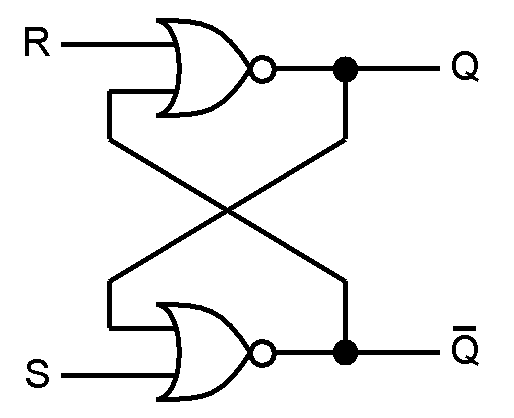
\includegraphics[width=0.45\textwidth]{imagens/SR-NOR-latch.png}
    \caption{Latch SR (set-reset) com portas NOR}
    \label{fig:latch}
\end{figure}

\begin{figure}[!h]
    \centering
    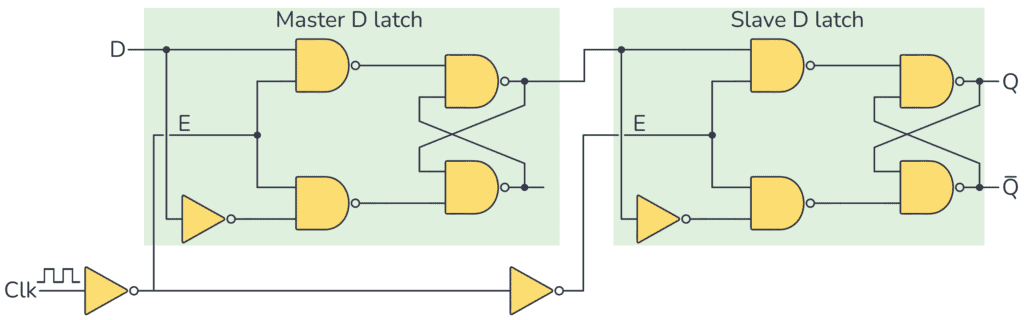
\includegraphics[width=0.8\textwidth]{imagens/Dflipflop-Master-Slave-edge-triggered-2-1024x320.png}
    \caption{Flip-flop tipo D mestre-escravo}
    \label{fig:ffTipoD}
\end{figure}

\begin{figure}[!h]
    \centering
    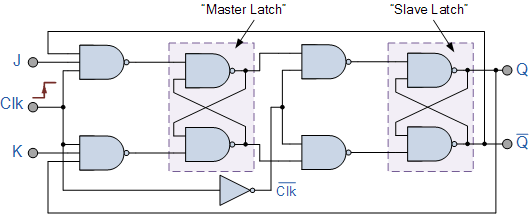
\includegraphics[width=0.8\textwidth]{imagens/sodapdf-converted.png}
    \caption{Flip-flop tipo JK mestre-escravo}
    \label{fig:ffTipoJK}
\end{figure}

O flip-flop JK possui quatro possíveis configurações de entrada: J=0 e K=0, J=0 e K=1, J=1 e K=0, e J=1 e K=1. Quando J e K são ambos 0, o flip-flop permanece no mesmo estado; quando J=0 e K=1, o estado do flip-flop é zerado; quando J=1 e K=0, o estado é invertido; e quando J e K são ambos 1, ocorre uma "alternância", ou seja, o estado atual é invertido para o estado oposto.

O flip-flop T é utilizado em contadores e sequenciadores que precisam de uma transição de estado a cada pulso do clock, enquanto o flip-flop D é mais utilizado em registradores e em circuitos de memória. O flip-flop JK é o mais versátil e pode ser utilizado em diversos tipos de circuitos, desde contadores até circuitos de controle de fluxo de dados.

Os flip-flops são fundamentais em eletrônica digital, permitindo a criação de circuitos complexos que processam e armazenam informações de forma precisa e confiável. O conhecimento dos diferentes tipos de flip-flops e suas características é essencial para o desenvolvimento de projetos eletrônicos avançados \cite{tocci2010sistemas}.

\section{Divisão de Frequência}
\label{divisorDeFrequencia}
Um divisor de frequência é um circuito eletrônico que reduz a frequência de um sinal de entrada, produzindo um sinal de saída com uma frequência mais baixa \cite{gouveia2017divisor}. Existem várias maneiras de projetar um divisor de frequência, mas uma abordagem comum é usar flip-flops para dividir a frequência.

Os flip-flops JK são um tipo de flip-flop que possuem duas entradas, J e K, além das entradas de clock e de saída. A entrada J é usada para definir o estado do flip-flop, enquanto a entrada K é usada para limpar o estado do flip-flop. Quando uma transição de subida do clock ocorre, o estado do flip-flop pode ser alterado com base nas entradas J e K.

Para projetar um divisor de frequência usando flip-flops JK, podemos conectar a saída de um flip-flop à entrada do clock do próximo flip-flop. A entrada J e K podem ser conectadas a uma fonte de sinal constante. Se for uma entrada ativa em todas as situações, sempre haverá comutação do estado, possibilitando a variação do clock. O clock do sistema é fornecido ao primeiro flip-flop, e a saída do último flip-flop é o sinal de saída do divisor de frequência. O número de flip-flops usados determina a taxa de divisão da frequência, sendo que cada flip-flop divide a frequência por 2.

Por exemplo, um divisor de frequência de 4 pode ser projetado usando dois flip-flops JK. A saída do primeiro flip-flop é conectada à entrada J do segundo flip-flop, e a entrada K de cada flip-flop é mantida em nível lógico "1". O sinal de entrada é fornecido à entrada de clock do primeiro flip-flop, e a saída do segundo flip-flop é o sinal de saída do divisor de frequência, que tem uma frequência quatro vezes menor do que a entrada.

Os divisores de frequência são amplamente utilizados em sistemas de comunicação, onde é comum ter que reduzir a frequência de um sinal para torná-lo mais adequado para transmissão ou processamento em outros componentes do sistema. Eles também são usados em instrumentação, em aplicações de áudio e em muitos outros tipos de circuitos eletrônicos. No protótipo descrito neste artigo, o mesmo haverá 2 utilizações: para obter um clock para o deslocamento dos bits e um para exibir os bits na matriz de LEDs. O clock do CLPD utilizado é de 50000000 Hz, ou 50 MHz. A seguinte equação representa o cálculo necessário para saber qual a frequência em relação a quantidade n de flip-flops:

\begin{equation} \label{Formula}
    x=\frac{50000000}{2^n}
\end{equation}

\section{Multiplexadores e matriz de LEDs}
O multiplexador é um componente eletrônico que permite selecionar um de vários sinais de entrada e direcioná-lo para a saída \cite{floyd}. Ele é usado para economizar espaço e reduzir a complexidade em sistemas digitais, permitindo que múltiplos sinais sejam roteados para um único canal de saída. O funcionamento de um multiplexador é relativamente simples: ele possui várias entradas e uma saída única. Além disso, ele tem um ou mais sinais de controle que determinam qual das entradas deve ser selecionada e enviada para a saída. No protótipo, ele será utilizado para passar os valores de cada coluna da matriz de LEDs e como bloco de seleção para o registrador de deslocamento universal. 

Por sua vez, uma matriz de LEDs é um conjunto de LEDs organizados em linhas e colunas, formando uma matriz bidimensional. Para acender um LED específico na matriz, é necessário selecionar a linha e a coluna correspondentes e enviar um sinal para a posição desejada. O uso de um multiplexador pode simplificar o processo de controle dos LEDs na matriz. Um multiplexador pode ser usado para selecionar a linha correta. Isso pode ser feito de forma rápida e eficiente, permitindo que os LEDs sejam controlados com precisão.

Para controlar uma matriz de LEDs, é necessário utilizar um microcontrolador ou outro dispositivo de processamento de sinal que possa enviar sinais para acionar cada LED individualmente. Esses sinais são geralmente fornecidos por meio de circuitos de driver de LED que amplificam o sinal de controle e o transmitem para os LEDs.

O processo de controle da matriz de LEDs envolve o envio de um sinal para as linhas e colunas específicas que correspondem aos LEDs que devem ser acesos. O microcontrolador envia um sinal para a linha e coluna apropriadas, fazendo com que o LED correspondente acenda.

A taxa de atualização da matriz de LED é importante para garantir que as imagens sejam exibidas com clareza e sem cintilação. Uma taxa de atualização rápida pode ser alcançada usando um sistema de multiplexação, onde as linhas são acionadas sequencialmente em rápida sucessão, criando uma ilusão de que todos os LEDs da matriz estão acesos ao mesmo tempo. O clock utilizado na matriz de LEDs, utilizando do divisor de frequência \ref{divisorDeFrequencia}, atinge 1,56Mhz.

\section{Registrador de Deslocamento}
Um registrador de deslocamento é um circuito digital que é utilizado para armazenar e deslocar bits em uma determinada direção \cite{tocci2010sistemas}. Um registrador de deslocamento construído com flip-flops do tipo D é chamado de registrador de deslocamento paralelo, pois todos os bits são transferidos em paralelo.

O registrador de deslocamento paralelo é construído com vários flip-flops do tipo D, conectados em série, com a saída de cada flip-flop conectada à entrada do próximo. A entrada de dados é conectada à entrada do primeiro flip-flop, e a saída é obtida a partir da saída do último flip-flop. Para deslocar os dados, um sinal de clock é aplicado em todos os flip-flops simultaneamente, fazendo com que os bits sejam transferidos para a direita ou para a esquerda, dependendo da direção do deslocamento.

Um registrador de deslocamento universal é um tipo de registrador de deslocamento que permite que os dados sejam enviados tanto da direita para a esquerda quanto da esquerda para a direita, utilizando multiplexadores. Esse tipo de registrador de deslocamento é construído com um número n de flip-flops e um número n de multiplexadores. Quando o sinal de controle do multiplexador é igual a 0, por exemplo, os dados são enviados para a direita, e quando o sinal de controle é igual a 1, os dados são enviados para a esquerda. O multiplexador seleciona a entrada correta, de acordo com a direção do deslocamento desejada.

Dessa forma, um registrador de deslocamento universal permite que os dados sejam deslocados em qualquer direção, dependendo do sinal de controle do multiplexador. Isso torna esse tipo de registrador de deslocamento mais flexível e versátil do que o registrador de deslocamento de deslocamento paralelo simples. 

\section{Contadores}
Contadores são circuitos digitais que são utilizados para contar pulsos de clock ou eventos em um sistema digital. Um contador pode ser construído utilizando flip-flops do tipo T, que são capazes de mudar de estado em cada pulso de clock. Existem vários tipos de contadores que podem ser construídos utilizando flip-flops do tipo T. Os contadores mais comuns são o contador binário, o contador BCD (binary coded decimal) e o contador de modulo \cite{floyd}.

O contador binário é o tipo mais simples de contador e é construído com flip-flops do tipo T conectados em cascata. Cada flip-flop é chamado de estágio do contador, e cada estágio representa um bit do número binário que está sendo contado. Quando um pulso de clock é aplicado, cada estágio muda seu estado de acordo com o valor do bit anterior. Por exemplo, se o contador estiver contando de 0 a 7, a sequência de estados dos flip-flops será 000, 001, 010, 011, 100, 101, 110 e 111.

O contador de modulo é utilizado para contar até um valor máximo, que é definido pelo número de estágios do contador. Ele é construído com flip-flops do tipo T conectados em cascata, com a saída do último flip-flop conectada à entrada do primeiro. O valor máximo que o contador pode contar é determinado pelo número de estágios. Por exemplo, um contador de modulo 8 pode contar de 0 a 7, enquanto um contador de modulo 16 pode contar de 0 a 15.

Em resumo, contadores construídos com flip-flops do tipo T são circuitos digitais simples e eficientes que podem ser utilizados em uma ampla variedade de aplicações, como sistemas de temporização, controle de acesso, medição de frequência e muito mais.